%
% $Id: main.tex 14 2014-02-04 22:36:30Z nicb $
%
\newcommand{\topic}{Campionamento, Sintesi ed Elaborazione dei Segnali Musicali\xspace}
\newcommand{\topicacro}{CSEDSM\xspace}
\newcommand{\level}{I\xspace}
\documentclass{scrbook}
\usepackage{graphicx}
\usepackage[italian]{babel}
\usepackage{svninfo}
\usepackage{fancyvrb}
\usepackage{paralist}
\usepackage[italian]{varioref}
\usepackage{nesse}
\usepackage{xspace}
\usepackage{needspace}
\usepackage{verbatim}
\usepackage{soul}

\newcommand{\imagedir}{./images}
\newcommand{\plotdir}{./plots}
\newcommand{\rcstag}{ver.\svnInfoRevision\ \svnInfoDate\xspace}
\newcommand{\cpholder}{Nicola Bernardini}
\newcommand{\cpyear}{2013}
\newcommand{\cpholderemail}{nicb@sme-ccppd.org}
\newcommand{\license}%
{%
  
\includegraphics{\imagedir/cc}
}

\title{%
	\topic (\topicacro) \level\\dispense\\{\tiny (\rcstag)}%
}
\author{Nicola Bernardini\\[2cm]\license}
\date{~}

\setlength{\parsep}{2\baselineskip}
\setlength{\parindent}{0pt}

\DeclareMathAlphabet{\mathpzc}{OT1}{pzc}{m}{it}

\begin{document}
\svnInfo $Id: main.tex 14 2014-02-04 22:36:30Z nicb $

\maketitle

\tableofcontents

\chapter{Introduzione\label{chap:introduction}}

%
% $Id: introduction.tex 14 2014-02-04 22:36:30Z nicb $
%

Queste sono le dispense della prima annualit\`a dell'insegnamento di \emph{\topic}
(aka \emph{\topicacro}) tenuto da Nicola Bernardini nell'A.A 2012-2013 al
Conservatorio ``C.Pollini'' di Padova.

Queste dispense sono tratte in larga parte da alcuni capitoli di \emph{A Digital Signal Processing Primer}
di Ken Steiglitz \cite{steiglitz:adspp} - integrati
con spiegazioni supplementari laddove l'aspetto matematico \`e pi\`u
complicato, e con materiali elaborati in
classe dagli studenti
nonch\'e tratti da altri testi
(cf. \cite{steiglitz1974introduction, t1987digital, park2010introduction, shenoi2005introduction}).


\chapter{Introduzione ai numeri complessi\label{chap:complex numbers}}

%
% $Id: complex.tex 14 2014-02-04 22:36:30Z nicb $
%
\svnInfo $Id: complex.tex 14 2014-02-04 22:36:30Z nicb $

\section{Cosa sono i numeri complessi?\label{sec:cosa}}

\begin{itemize}

	\item qual'\`e il risultato dell'equazione $x^2 + 1 = 0$?

	\item per trovare la soluzione a questa domanda i matematici hanno esteso il
	dominio dei numeri reali con i numeri \emph{immaginari}, detti anche numeri
	\emph{complessi}

  \item propriet\`a dei numeri complessi:

		\begin{itemize}
	
	  	\item si tratta di numeri bidimensionali
	          (costituiti di due parti, una parte reale e una parte \emph{immaginaria})

			\item si possono immaginare quindi come numeri che invece di trovarsi su
						una retta si trovano su un piano

			\item pertanto si perde la possibilit\`a di \emph{ordinarli} in maniera
			      semplice ($==$ non ha senso dire che ``un numero complesso \`e
						pi\`u grande o pi\`u piccolo di un altro'')

			\item operazioni sui numeri complessi:

					\begin{description}

					  \item[coniugazione] il \emph{complesso coniugato} di un
						numero complesso \`e lo stesso numero con la parte immaginaria
						invertita:

							\begin{equation}
								z = x + i y, \bar{z} = x - i y
							\end{equation}

						la moltiplicazione di un numero complesso con il suo complesso
						coniugato d\`a luogo a un numero reale che \`e il quadrato della
						parte reale sommato al quadrato della parte immaginaria

		          \begin{equation}
							 	z \bar{z} = ( x + i y ) ( x - i y ) = x^2 + y^2 + i x y - i x y = x^2 + y^2
		          \end{equation}
						

						\item[addizione/sottrazione] si aggiungono
						e si sottraggono separatamente: parte reale con parte reale e parte immaginaria con parte immaginaria 
						\item[moltiplicazione] si moltiplicano come nella moltiplicazione
						di binomi, ricordando per\`o che $i^2 = -1$:

						\begin{equation}
						   a = x_1 + iy_1,\quad b = x_2 + iy_2\quad\\
							 a \times b = x_1 x_2 - y_1 y_2 + i \left ( x_1 y_2 x_2 y_1 \right )
		        \end{equation}

						\item[divisione] le divisioni sono definite negli termini delle
						moltiplicazioni, moltiplicando entrambi i fattori per il complesso
						coniugato del denominatore:

						\begin{equation}
						   z_1 = x_1 + i y_1,\quad z_2 = x_2 + i y_2
		 				\end{equation}
		 				\begin{equation}
							 \frac{z_1}{z_2} = \frac{x_1 + i y_1}{x_2 + i y_2}
		         \end{equation}
		         \begin{equation}
							 \frac{(x_1 + i y_1) \times (x_2 - i y_2)}{(x_2 + i y_2) \times (x_2 - i y_2)}\\
							 = \left ( \frac{x_1 x_2 + y_1 y_2 }{x_2^2 + y_2^2} \right ) + i \left ( \frac{y_1 x_2 - x_1 y_2}{x_2^2 + y_2^2} \right )
		 				\end{equation}
		 				\begin{equation}
							 \frac{(x_1 x_2 + y_1 y_2) - i (y_1 x_2 + x_1 y_2)}{x_2^2 + y_2^2}
		        \end{equation}

					\end{description}

			\end{itemize}
							
\end{itemize}

\section{Le scomposizioni in serie}

\begin{itemize}

  \item come si calcolano al computer i valori di
    $e^x$, $sin(x)$, $cos(x)$, ecc.?

	\item si calcolano in forma approssimata \emph{scomponendoli in serie}:

		\begin{equation}
    	  e^x = 1 + x + \frac{x^2}{2!} + \frac{x^3}{3!} + \frac{x^4}{4!} + \ldots + \frac{x^n}{n!}
		\end{equation}
		\begin{equation}
       sin(x) = x - \frac{x^3}{3!} + \frac{x^5}{5!} - \frac{x^7}{7!} + \ldots
		\end{equation}
		\begin{equation}
       cos(x) = 1 - \frac{x^2}{2!} + \frac{x^4}{4!} - \frac{x^6}{6!} + \ldots
		\end{equation}

    se si usano i numeri complessi, si ottiene la formula di Eulero:

		\begin{equation}
    	e^{ix} = cos(x) + i sin(x)
		\end{equation}

		(ossia sommando le scomposizioni in serie di $cos(x)$ e $i sin(x)$ e
		si ottiene la scomposizione in serie di $e^x$)

		dato che $i = 0 + i$, $i^2 = -1$, $i^3 = 0 - i$, $i^4 = 1$, $i^5 = i$, $i^6 = -1$, ecc.

    quindi: $e^x$ va all'infinito, ma $e^{ix}$ oscilla tra $+1$ e $-1$

    dato che anche $i^n$ oscilla invece di andare all'infinito

\end{itemize}

\section{Altre propriet\`a dei numeri complessi}

\begin{itemize}

  \item parte reale:

		\begin{equation}
			z = x + i y\nonumber
		 \end{equation}
		 \begin{equation}
			Re(z) = x
		\end{equation}

	\item parte immaginaria:

		\begin{equation}
			z = x + i y\nonumber
		 \end{equation}
		 \begin{equation}
			Im(z) = y
		\end{equation}

    attenzione! la ``parte immaginaria'' di un numero complesso \`e costituita
		da un numero \emph{reale}, il quale viene a sua volta moltiplicato per
		l'operatore immaginario $i$
		

  \item modulo: la ``distanza dal centro'', ossia la somma del quadrato della
	parte reale con il quadrato della parte immaginaria sotto radice:

		 \begin{equation}
		 	z = x + i y\nonumber
		 \end{equation}
		 \begin{equation}
			abs(z) = \sqrt{x^2 + y^2}
		 \end{equation}

		 nel caso di fenomeni periodici, \emph{modulo} e \emph{magnitudine} sono
		 sinonimi

	\item argomento: l'angolo costituito dal numero complesso rispetto all'asse
	reale

		\begin{equation}
		 	z = x + i y\nonumber
		 \end{equation}
		 \begin{equation}
			arg ( z ) = \angle{z} = atan \left ( \frac{Im(z)}{Re(z)} \right ) = atan \left ( \frac{y}{x} \right )
		\end{equation}
	
		 nel caso di fenomeni periodici, \emph{argomento} e \emph{fase} sono
		 sinonimi

\end{itemize}

\subsection{Esercizi}

\begin{itemize}

  \item rifare la dft con $e$ invece che con $sin$/$cos$
  \item verificare la giustezza della fase 

\end{itemize}

\section{Fasori complessi (cf.\cite[2.4 p.40]{steiglitz1974introduction})}

\begin{itemize}

  \item Abbiamo visto che un oscillatore cosinusoidale pu\`o essere rappresentato come
segue:

\begin{equation}
  F(k) = A cos(\omega k + \phi)\quad \textrm{dove}\,k\,\textrm{\`e un intero}
\end{equation}

(fare il plot di $F(k)$ per valori non--negativi di $k$)

  \item secondo la formula di Eulero,
	
		 \begin{equation}
				F(k) = Re \left ( A e^{i(\omega k + \phi)} \right )
		 \end{equation}

	\item mentre un oscillatore sinusoidale $F(k) = A sin ( \omega k + \phi)$
					corrisponde a
	
		 \begin{equation}
				F(k) = Im \left ( A e^{i(\omega k + \phi)} \right )
		 \end{equation}

	\item quindi $A e^{i(\omega k+ \phi)}$ \`e un \emph{fasore complesso}

  \item interpretazione grafica:
	
		\begin{itemize}

			\item un punto che si muove su un cerchio sul piano
  complesso: A \`e il raggio del cerchio. k sono i punti crescenti sul cerchio

			\item parte reale: coseno campionato

			\item parte immaginaria: seno campionato

			\item $\phi$ \`e il punto di partenza (la fase)

		\end{itemize}

	\item se $\phi = 0$ e $\omega = 0$, il fasore rimane fermo al punto di partenza e $F(k) = A$ (costante reale)

  \item alla fine del giro il fasore ricomincia perch\'e:

		\begin{equation}
  		e^{i(\omega k+ \phi)} = e^{i(\omega k + \phi + 2 \pi)}
		\end{equation}

\end{itemize}

\section{Rivisitando \emph{nyquist} e \emph{foldover} con i fasori complessi}

\begin{itemize}

	\item cosa succede se $\omega = \pi$?

  \item e se $\omega > \pi$?
	
	\item mettiamo conto che $\omega = \pi + x$:

		 \begin{equation}
        e^{i\omega k} = e^{i(\pi + x)k}
		 \end{equation}

  dato che $e^{i(2 \pi k)} = 1$ possiamo aggiungere o togliere $2\pi$ al nostro
  fasore a piacere:

		 \begin{equation}
       e^{i\omega k} = e^{i(\pi + x)k} = e^{i(-2\pi + \pi + x)k} = e^{i(-\pi + x)k}
		 \end{equation}

  quindi sembra che il fasore stia andando all'indietro (effetto stroboscopico)

\end{itemize}


\chapter{I filtri FIR\label{chap:fir}}

%
% $Id: FIR.tex 14 2014-02-04 22:36:30Z nicb $
%

\section{Un filtro FIR semplice\label{sec:simple fir}}

\subsection{Dominio continuo di tempo\label{sec:continuous time}}

Nei filtri FIR (\emph{feed-forward}) l'output \`e la somma dell'input e una versione riscalata e ritardata
		dell'input:

		\begin{equation}\label{eqn:fir semplice}
						y_t = x_t + a_1 x_{t-\tau}
			\end{equation}

		(aggiungere grafico)

	Poniamo che $x_t$ sia un segnale sinusoidale complesso:

		 \begin{equation}
	    x_t = e^{i\omega t}\nonumber
		 \end{equation}

		 \begin{equation}
			y_t = e^{i \omega t} + a_1 e^{i \omega (t - \tau)}
		 \end{equation}

		(fare schemino sul cerchio unitario)

		 \begin{equation}
		  y_t = e^{i \omega t} + a_1 e^{i \omega t} e^{-i \omega \tau} = e^{i\omega t} \left [ 1 + a_1 e^{-i \omega \tau} \right ]
		 \end{equation}

	Quindi l'uscita \`e sempre un fasore di frequenza $\omega$ moltiplicato per
		un'ampiezza che \`e funzione di $\omega$ (ma indipendente dal tempo!)

	La funzione del filtro \`e dunque $\left [ 1 + a_1 e^{-i \omega \tau} \right ]$ e la chiameremo $H(\omega)$

	Per capire la risposta in frequenza e in fase dobbiamo capire che $H(\omega)$ \`e
		in realt\`a la magnitudine (valore assoluto di $H(\omega)$ moltiplicata per una
		funzione della fase:

		 \begin{equation}
		  H(\omega) = |H(\omega)| e^{i \Theta(\omega)}
		 \end{equation}

	 dove $|H(\omega)| = |1 + a_1 e^{-i\omega \tau}|$; siccome per il teorema di Pitagora il
	 modulo \`e il quadrato della parte reale + il quadrato della parte
	 immaginaria sotto radice,

		 \begin{equation}
	  Re(H(\omega)) = 1 + a_1 cos(\omega \tau)
		 \end{equation}
		 \begin{equation}
		Im(H(\omega)) = - a_1 sin(\omega \tau)
		 \end{equation}

		 \begin{equation}
	  Re^2 = 1 + 2 a_1 cos(\omega \tau) + a_1^2 cos^2(\omega \tau)
		 \end{equation}
		 \begin{equation}
		Im^2 = a_1^2 sin^2(\omega \tau)
		 \end{equation}

		quindi
		
		 \begin{equation}
		Re^2 + Im^2 = 1 + 2 a_1 cos(\omega \tau) + a^2 [ cos^2(\omega \tau) + sin^2(\omega \tau) ]
		 \end{equation}

		 Dato che

		 \begin{equation}
				cos^2(\alpha) + sin^2(\alpha) = 1
		 \end{equation}

		 per $\alpha$ qualsiasi,

		 \begin{equation}
				1 + 2 a_1 cos(\omega \tau) + a^2 [ cos^2(\omega \tau) + sin^2(\omega \tau) ] = 1 + 2 a_1 cos(\omega \tau) + a^2
		 \end{equation}
		 \begin{figure}[htb]
			 \begin{center}
					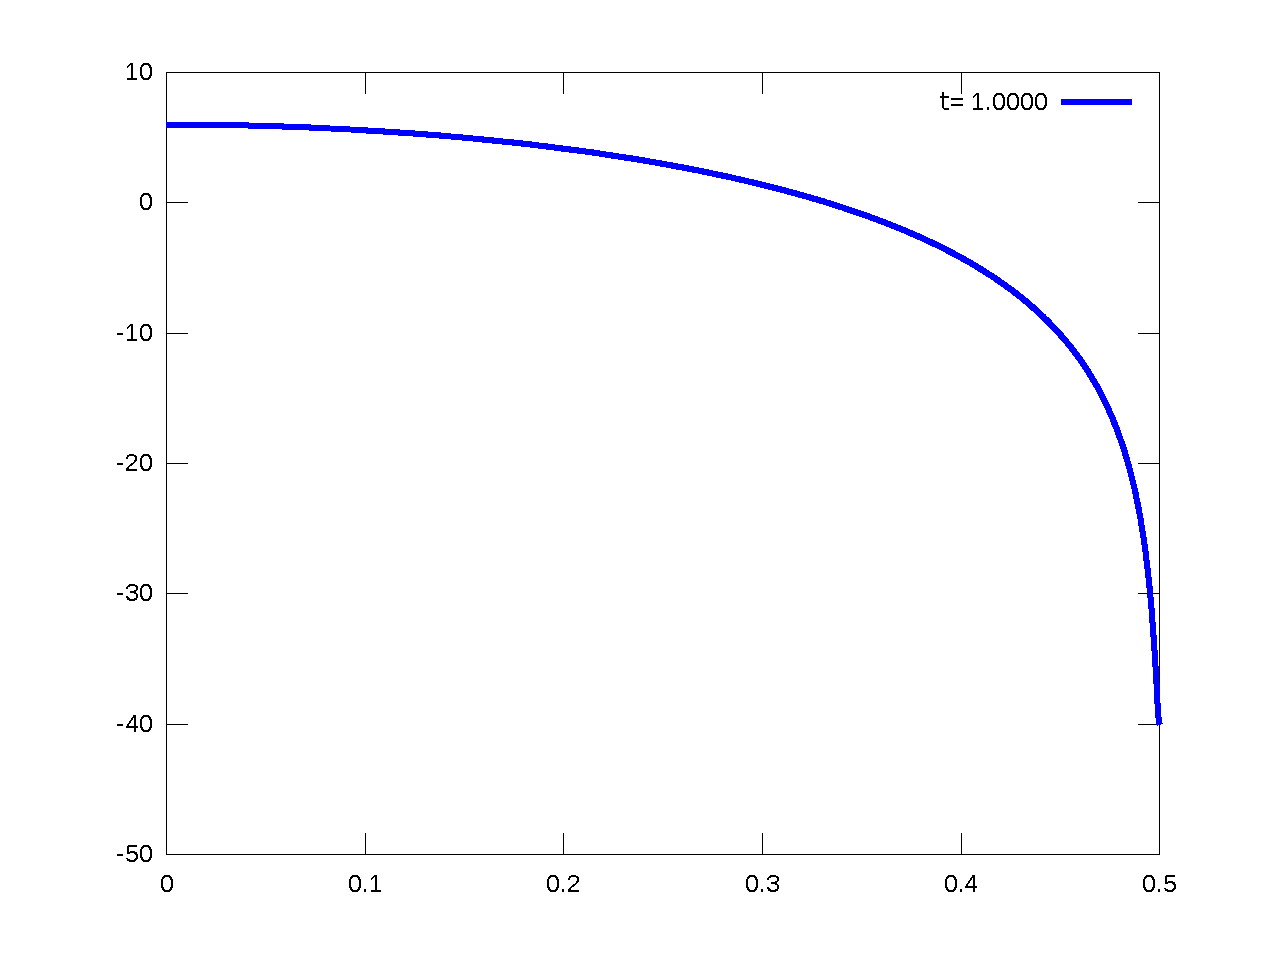
\includegraphics[width=0.8\textwidth]{\plotdir/fir2}
					\caption{Filtro FIR con $\tau = 1/fc$\label{fig:fir con tau 1}}
			 \end{center}
		 \end{figure}
		 \begin{figure}[htb]
			 \begin{center}
					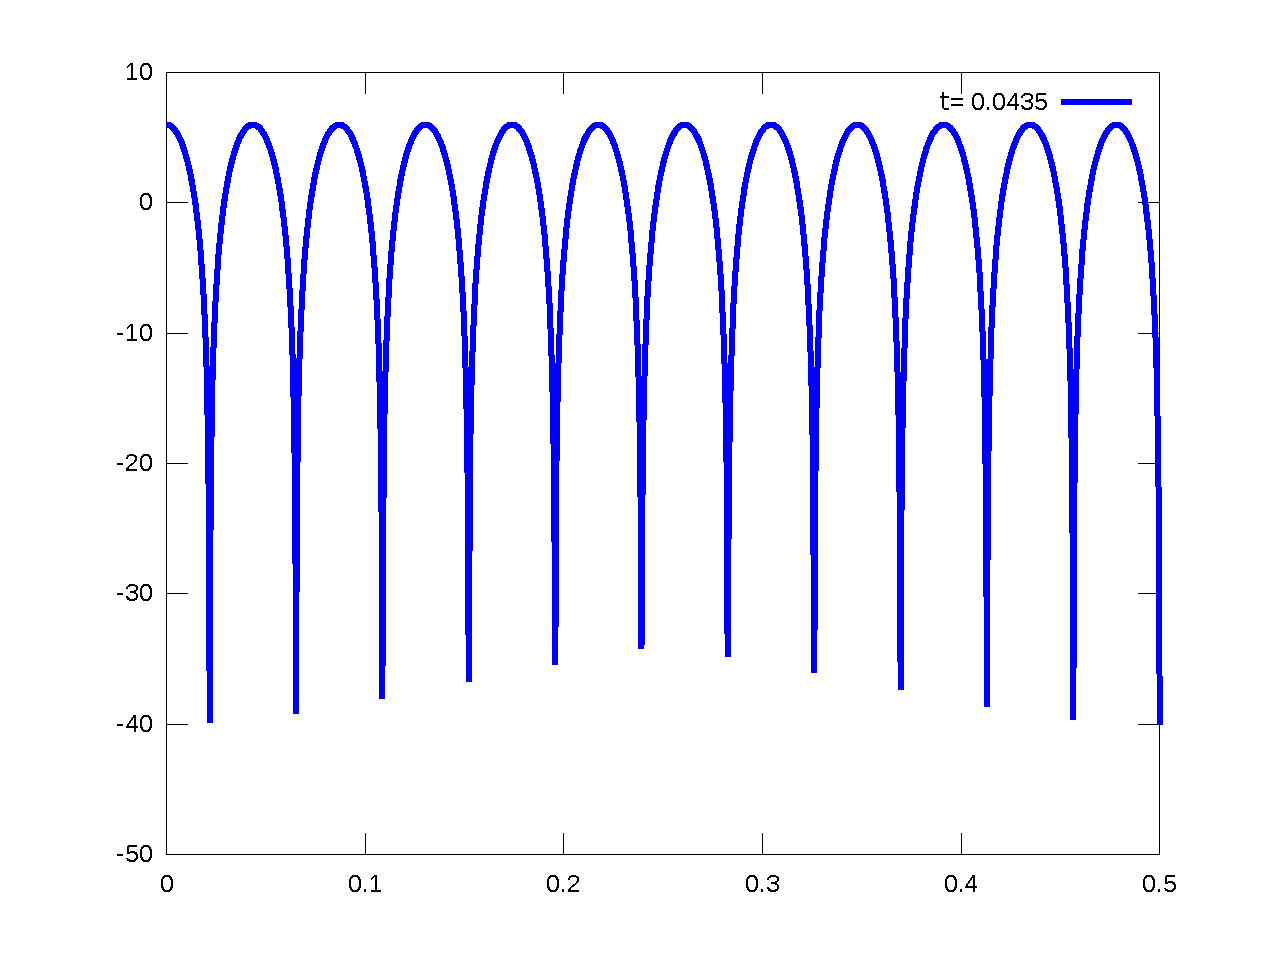
\includegraphics[width=0.8\textwidth]{\plotdir/fir3}
					\caption{Filtro FIR con $\tau = 23/fc$\label{fig:fir con tau 23}}
			 \end{center}
		 \end{figure}
		 Le Figg.\vref{fig:fir con tau 1} e \vref{fig:fir con tau 23} mostrano la
		 risposta in frequenza rispettivamente per $\tau = 1/fc$ e per $\tau = 23/fc$.

\subsection{Esercizi}

\begin{itemize}

	\item fare il plot della risposta in frequenza con vari valori di $\omega$ e
					di $\tau$

\end{itemize}


\subsection{Passaggio dal tempo continuo al tempo discreto}


	Il ritardo $\tau$ viene ristretto ad un numero intero di campioni multiplo della
		periodo di campionamento $T_s$ (restrizione)

	Dato che la frequenza di campionamento interesser\`a  la  definizione
    del  nostro  segnale  (per  le  frequenze  che   servono   per   una
    applicazione piuttosto che un'altra), ma non  il  funzionamento  del
    filtro, possiamo  benissimo  normalizzare  la  nostra  frequenza  di
    campionamento a $1$, avendo cos\`i la frequenza di Nyquist a $0.5$

	Ora, se noi ritardiamo il nostro segnale di un campione (invece che del
		valore continuo tau) moltiplicheremo il nostro fasore in ingresso per
		$e^{-i \omega T}$ dove $\omega T$ \`e l'angolo in radianti per campione. Possiamo sempre
		ricavare il tempo nel dominio digitale moltiplicando per il periodo di
		campionamento $T_s$ - possiamo quindi evitare di scrivere $T_s$, che diventa
		una sorta di costante di conversione: se la costante \`e 1 (frq di
		campionamento 1) possiamo evitare di scriverla ogni volta

	La frequenza di campionamento diventa $\omega = 2 \pi$ e la frequenza di nyquist \`e
		$\omega = \pi$ radianti per campione e il nostro fasore sar\`a sempre

		 \begin{equation}
	 			x_t = e^{i\omega kT}
		 \end{equation}
		
		dove $k$ \`e un numero intero di campioni e $T$ \`e il periodo di campionamento

		Ora rifacciamo il filtro dell'eq.\ref{eqn:fir semplice} della Sez.\vref{sec:continuous time} ritardando per\`o non di tau
	  ma di un solo campione:

		 \begin{equation}
		   y_k = x_k + a_1 x_{k-1}
		 \end{equation}

	  applicando il fasore digitale, il filtro diventer\`a:

		 \begin{equation}
	  	  y_k = e^{i\omega kT} [ 1 + a_1 e^{-i\omega \times 1} ] = e^{i \omega kT} [ 1 + a_1 e^{-i \omega } ]
		 \end{equation}

		e la magnitudine (== risposta in frequenza) sar\`a:

		 \begin{equation}
		  |H( \omega )| = 1 + 2 a_1 cos( \omega ) + a_1^2
		 \end{equation}

	Ricapitolando, se l'input di un filtro FIR \`e il fasore $e^{i \omega kT}$

		 \begin{equation}
	   y_t = a_0 x_t + a_1 x_{t-1}
		 \end{equation}

    (ritardo di un campione).

		L'output \`e anche un fasore con frequenze inalterate

		 \begin{equation}
		 y_k = x_k \left [ a_0 + a_1 e^{-i \omega} \right ]
		 \end{equation}

		possiamo aggiungere quanti termini vogliamo in un filtro del genere:

		 \begin{equation}
		 y_k = x_k \left [ a_0 + a_1 e^{-i\omega } + a_2 e^{-i2\omega } + a_3 e^{-i3\omega } + ... + a_n e^{-in\omega } \right ]
		 \end{equation}


	Invece di ripetere $e^{i\omega}$ ogni volta, possiamo operare una sostituzione: sostituiamo $z = e^{i \omega}$

	Il ritardo di un campione diventa cos\`i $z^{-1}$, e il ritardo di $k$ campioni
		diventa cos\`i $z^{-k}$

	$z^{-1}$ \`e trattabile sia come una variabile complessa che come un
		operatore, cio\`e una operazione applicata ad un certo oggetto (pensate
		p.es. ad un operatore che ruota un disegno di 90 gradi) $= \rho$: $\rho^2$ lo
		ruota di 180 gradi in senso antiorario, $\rho^{-1}$ lo ruota in senso orario)

	Possiamo anche usare la notazione $X$ per rappresentare un \emph{intero segnale}
		(un vettore di campioni); nota bene: $x_k$ rappresenta il valore di un
		segnale al tempo $k$, $X$ rappresenta \emph{l'intero segnale}.

	L'intero segnale ritardato di un campione \`e quindi notato $z^{-1} X$ quindi
		significa ``applica l'operatore $z^{-1}$ al segnale $X$''

		L'equazione si riscrive:

		 \begin{equation}
		  Y = a_0 X + a_1 z^{-1} X = \left [ a_0 + a_1 z^{-1} \right ] X
		 \end{equation}

		(nota che anche l'ampiezza diventa un operatore: moltiplica \emph{tutto il
		segnale} per la costante $a_0$, e quest'operatore \`e commutativo).

	Quindi $Y = H(z) X$ dove $H(z) = a_0 + a_1 z^{-1}$.

% \item se del caso fare due filtri in cascata moltiplicando le funzioni di
% 	trasferimento

\subsection{Esercizi}

\begin{enumerate}

	\item Si descriva un filtro FIR con l'equazione che segue:

					\begin{equation}
						y_k = x_k + x_{k-1} + x_{k-2} + \ldots + x_{k-19}
					\end{equation}

				Si derivi una espressione algebrica semplice per la sua risposta in
				magnitudine. Si trovi quali siano le frequenze alle quali si trovano
				dei picchi e quelle alle quali si trovano dei buchi

\end{enumerate}


\chapter{Funzioni di variabile complessa\label{chap:complex variable functions}}

%
% $Id: piano_z.tex 14 2014-02-04 22:36:30Z nicb $
%
\svnInfo $Id: piano_z.tex 14 2014-02-04 22:36:30Z nicb $

\section{Il piano Z\label{sec:pianoz}}

La rappresentazione delle caratteristiche della funzione di trasferimento di
un filtro sul \emph{piano z} complesso permette di capirne meglio il
funzionamento.

Riprendiamo il nostro filtro semplice

\begin{equation}\label{eq:simple fir}
	y_t = x_t - a_1 x_{t-1}
\end{equation}

Se sostituiamo in \ref{eq:simple fir} $x_t$ con un fasore, l'effetto di questo
filtro equivale alla moltiplicazione dell'ingresso per la funzione complessa

\begin{equation}\label{eq:simple transf function}
	1 - a_1 e^{-i \omega} = 1 - a_1 z^{-1}
\end{equation}

perch\'e abbiamo introdotto la stenografia $z = e^{i \omega}$.

Abbiamo quindi una funzione di trasferimento complessa  $\mathpzc{H} ( z )$
alla quale corrisponde la risposta in frequenza

\begin{equation}\label{eq: complex freq response}
		H ( \omega ) = \mathpzc{H} ( e^{i \omega} )
\end{equation}

In sostanza, la risposta in frequenza \`e la funzione di trasferimento della
variabile complessa $z$ \emph{valutata sul cerchio unitario}.
I valori di $\omega$ che ci interessano vanno da $\omega = 0$ alla frequenza
di Nyquist $\omega = \pi$ radianti per campione. Si tratta quindi della met\`a
superiore del cerchio nel piano $z$, come illustrato in Fig.\vref{fig: z plane frequency axis}
\begin{figure}[htp]
\begin{center}
	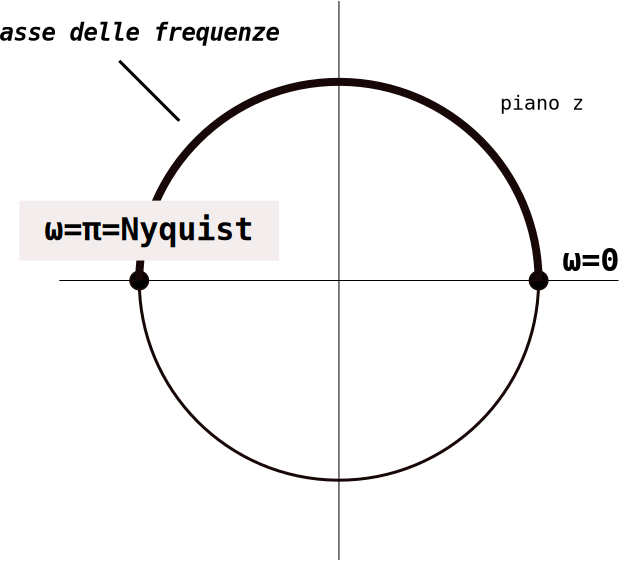
\includegraphics[width=0.4\textwidth]{\imagedir/frequency_axis_z_plane}
	\caption{L'asse delle frequenze sul piano $z$.\label{fig: z plane frequency axis}}
\end{center}
\end{figure}

Ora guardiamo pi\`u attentamente la funzione di trasferimento del nostro
esempio. Essa \`e

\begin{equation}\label{eq: simple transfer function 2}
				\mathpzc{H} ( z ) = 1 - a_1 z^{-1}
\end{equation}

Riscriviamola ora come rapporto di polinomi moltiplicando sopra e sotto per $z$:

\begin{equation}\label{eq: simple transfer function 3}
				\mathpzc{H} ( z ) = 1 - a_1 z^{-1} = \frac{z}{z} - \frac{a_1}{z} = \frac{z - a_1}{z}
\end{equation}

In questo modo appaiono chiaramente le radici dell'equazione:
c'\`e uno zero nel numeratore a $z = a_1$ e uno zero nel denominatore a $z = 0$. Vale a dire:
la funzione di trasferimento diventa zero a $z = a_1$ e infinita per $z = 0$.
La magnitudine della risposta in frequenza \`e la magnitudine di $\mathpzc{H} ( z )$
calcolata sul cerchio unitario (cio\`e quando $z = e^{i \omega}$):

\begin{equation}\label{eq: simple magnitude}
	| H ( \omega ) | = \frac{| z - a_1 |}{| z |}
\end{equation}

$| z | = 1$ perch\'e ci troviamo sul cerchio unitario (dato che $z = e^{i \omega}$).
In effetti, nei filtri \emph{feed-forward} (FIR) gli unici zeri al
denominatore possono apparire solo all'origine, e non hanno quindi alcun
effetto sulla risposta in frequenza. Possiamo quindi riscrivere l'Eq.\ref{eq: simple magnitude}
cos\`i:

\begin{equation}\label{eq: simple magnitude rewritten}
				| H ( \omega ) | = | z - a_1 |~\text{per}~z = e^{i \omega}
\end{equation}
\begin{figure}[htp]
\begin{center}
				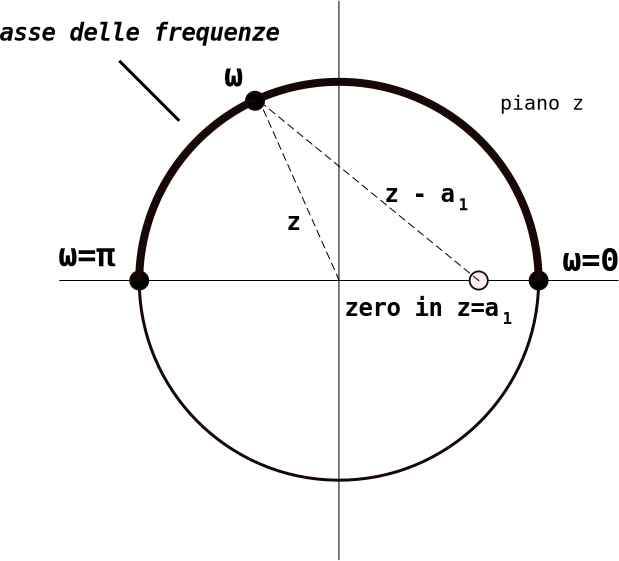
\includegraphics[width=0.4\textwidth]{\imagedir/mag_response}
				\caption{Valutazione della risposta in magnitudine per $z = e^{i
				\omega}$. Il fattore $|z - a_1|$ \`e la lunghezza del vettore dallo
				zero in $a_1$ sino al punto sul cerchio unitario corrispondente alla
				frequenza $\omega$\label{fig:mag response}}
\end{center}
\end{figure}

Ecco il significato della figura \ref{fig:mag response}: immaginiamo di
camminare sul cerchio unitario da $\omega = 0$ sino a $\omega = \pi$.
Quando ci troveremo vicino a $\omega = 0$, il modulo del vettore $|z - a_1|$
sar\`a molto piccolo e quindi influir\`aà molto sulla magnitudine del 
della funzione di trasferimento (riducendola). Man mano che ci allontaneremo
da $\omega = 0$ il modulo aumenter\`a e di conseguenza anche la magnitudine
della funzione di trasferimento. Quindi \`e ovvio che la Fig.\vref{fig:mag
response} ci sta mostrando la funzione di trasferimento di un filtro
passa--alto. Mentre per $a_1$ negativi si avrebbe un filtro passa--basso.
\begin{figure}[htp]
\begin{center}
				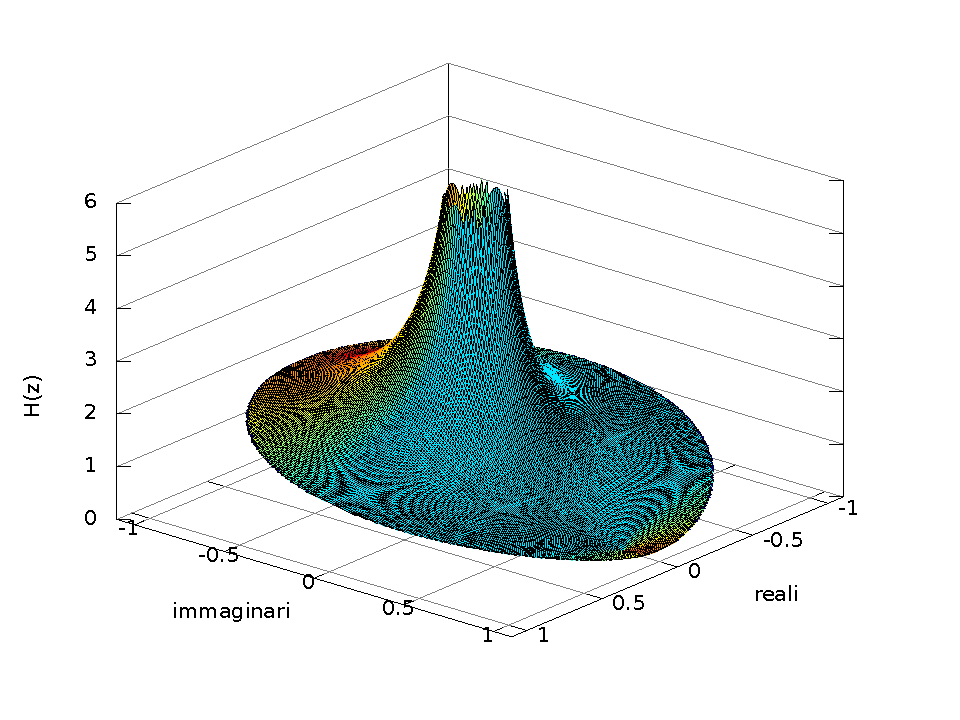
\includegraphics[width=0.85\textwidth]{\plotdir/zplane}
				\caption{La funzione $|\mathpzc{H}(z)|$ sul piano $z$\label{fig:mag response z plane}}
\end{center}
\end{figure}

La figura \vref{fig:mag response z plane} illustra la magnitudine della
funzione $z$ all'interno del cerchio unitario per $a_1 = 0.8$.


% completare la sezione


\chapter{La risposta in fase dei filtri FIR\label{chap:FIR phase response}}

%
% $Id: fase.tex 14 2014-02-04 22:36:30Z nicb $
%
% p.76 cap.4 n.7
%
\svnInfo $Id: fase.tex 14 2014-02-04 22:36:30Z nicb $

\section{La risposta in fase\label{sec:phase}}

Riconsideriamo ancora una volta il filtro che abbiamo analizzato in
Cap.\ref{chap:fir} Sez.\vref{sec:simple fir} (eq.\ref{eqn:fir semplice}):

		\begin{equation}\label{eqn:fir semplice 2}
						y_t = x_t + a_1 x_{t-\tau}
			\end{equation}

la cui risposta in frequenza \`e una funzione della frequenza $\omega$

	\begin{equation}\label{eqn:fir semplice frqresp}
	       H ( \omega ) = 1 + a_1 e^{-i \omega}
	\end{equation}

Questa risposta complessa in frequenza avr\`a quindi una magnitudine e un
angolo per ciascun $\omega$. Cio\`e l'eq.\ref{eqn:fir semplice frqresp} pu\`o
essere riscritta come 

	\begin{equation}\label{eqn:fir semplice frqresp 2}
	       1 + a_1 e^{-i \omega} = |H ( \omega )| e^{i \Theta ( \omega )}
	\end{equation}

Se il segnale in ingresso fosse un fasore complesso $x = e^{i \omega t}$,
il fasore in uscita $y$ sarebbe il prodotto di questo ingresso moltiplicato
questa funzione di trasferimento

	\begin{equation}\label{eqn:fs output}
		y_t = |H ( \omega )|e^{i (\omega t + \Theta ( \omega ) )}
	\end{equation}

il che significa che l'uscita \`e una copia dell'ingresso ritardata in fase di
un angolo $\Theta ( \omega )$ e riscalata in ampiezza di $| H ( \omega )|$.

Per capire quanto valga il ritardo di fase possiamo usare la funzione
\emph{arcotangente}. Riscrivendo l'eq.\ref{eqn:fir semplice frqresp} come $1 +
a_1 cos \omega - i a_1 sin \omega$, avremo

  \begin{equation}\label{eqn:risp in fase}
			\begin{array}{r c l}
							\Theta ( \omega ) & = & arctan \left [ \frac{\mathpzc{Immag} H ( \omega )}{\mathpzc{Reale} H ( \omega )} \right ]\\
							                  & = & arctan \left [ \frac{- a_1 sin \omega}{1 + a_1 cos \omega} \right ]\\
			\end{array}
	\end{equation}

Quando $a_1 = 1$ l'espressione contenuta in eq.\ref{eqn:risp in fase} si
semplifica. Riscrivendo la funzione di trasferimento di eq.\ref{eqn:fir semplice frqresp}
con $a_1 = 1$:

	\begin{equation}\label{eqn:fir semplice frqresp 3}
			H ( \omega ) = 1 + e^{-i \omega} = e^{-i \omega / 2} \left [ e^{i \omega / 2} + e^{-i \omega / 2} \right ]
	\end{equation}

Ricordiamo che la formula di Eulero $e^{i \alpha} = cos \alpha + i sin
\alpha$, e che quindi

	\begin{equation}\label{eqn:remember eulero}
			\begin{array}{r c l}
							cos \alpha & = & \frac{e^{i \alpha} + e^{-i \alpha}}{2}\\
							sin \alpha & = & \frac{e^{i \alpha} - e^{-i \alpha}}{2i}\\
							e^{i \alpha} + e^{-i \alpha} & = & 2 cos \alpha\\
							e^{i \omega / 2 } + e^{-i \omega / 2} & = & 2 cos \omega / 2\\
			\end{array}
	\end{equation}

	allora l'eq.\ref{eqn:fir semplice frqresp 3} si semplifica in

  \begin{equation}\label{eqn:fir semplice frqresp 3 result}
		H (\omega) =  e^{-i \omega / 2} 2 cos (\omega / 2)\\
	\end{equation}

Confrontando l'eq.\ref{eqn:fir semplice frqresp 2} con la \ref{eqn:fir semplice frqresp 3 result},
$2 cos (\omega / 2)$ \`e la magnitudine della risposta (reale) $|H ( \omega )|$,
mentre l'esponenziale complesso $e^{-i \omega / 2}$ \`e la risposta in fase
e rappresenta un ritardo di fase di un angolo $- \omega / 2$.
Quindi, se l'ingresso \`e il fasore $e^{i \omega t}$, l'uscita del filtro
sar\`a il fasore

	\begin{equation}\label{eqn:fir output}
			2 cos ( \omega / 2 ) e^{i \omega (t - 1 / 2)}
	\end{equation}

il che equivale a dire che l'effetto del filtro sulla fase del segnale \`e
quello di ritardarlo esattamente di un tempo equivalente alla met\`a della
frequenza di campionamento, \emph{indipendentemente dalla frequenza} $\omega$
\emph{del fasore in ingresso}.

Questo \`e un caso speciale di una caratteristica importante dei filtri FIR:
se i coefficienti di un filtro FIR sono simmetrici intorno al proprio centro
(in questo caso i coefficienti sono $\{ 1, 1 \}$, la risposta in fase \`e
proporzionale ad $\omega$, trattandosi quindi di un ritardo di tempo fisso per
tutte le frequenze. Il filtro si dice quindi \emph{a fase lineare}, ossia non
introduce distorsioni nella risposta in fase.

La fig.\vref{fig: fase 3} riporta la risposta in frequenza e la risposta in
fase del filtro FIR

\begin{equation}\label{eqn: fir 3}
	H ( z ) = 0.5 - 0.8 z^{-1} + 0.5 z^{-2}
\end{equation}
\begin{figure}[htb]
	\begin{center}
	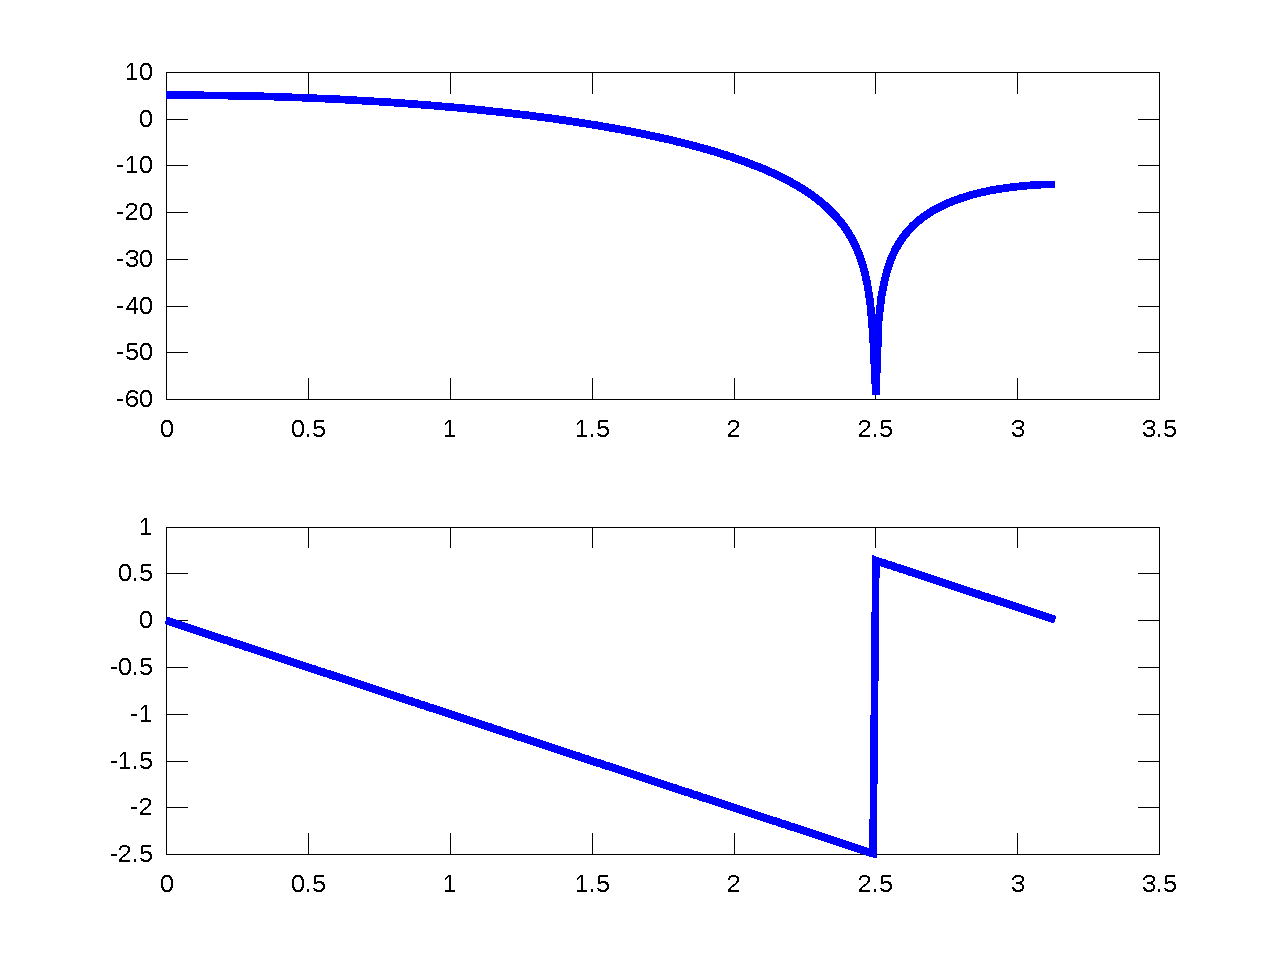
\includegraphics[width=0.9\textwidth]{\plotdir/fase_3}
	\caption{Risposta in frequenza e in fase del filtro la cui funzione di
	trasferimento \`e riportata in eq.\ref{eqn: fir 3}\label{fig: fase 3}}
	\end{center}
\end{figure}

Come si pu\`o notare, un numero dispari di coefficienti genera una risposta in
fase lineare.

Lo script {\tt octave} che genera questa figura \`e riportato qui:

\verbatiminput{\plotdir/fase_3.m}


\chapter{I filtri comb inversi\label{chap:icf}}

%
% $Id: icf.tex 14 2014-02-04 22:36:30Z nicb $
%
% p.77 cap.4 n.8
%
\svnInfo $Id: icf.tex 14 2014-02-04 22:36:30Z nicb $

\section{Introduzione ai filtri comb inversi\label{sec:icf introduction}}

I filtri comb inversi sono un caso particolare di filtri FIR. Essi permettono,
ad esempio, di cancellare le componenti di un segnale armonico.

Si tratta come sempre di un filtro FIR come quello studiato in
Sez.\ref{sec:simple fir}.\vref{sec:continuous time}  (eq.\ref{eqn:fir
semplice}). Sostituiamo al posto del ritardo arbitrario $\tau$ un numero
intero di campioni $L$. Come coefficiente del filtro prenderemo $R^{L}$.

L'equazione diventer\`a quindi

\begin{equation}\label{eqn:icf 1}
		y_t = x_t - R^{L} x_{t - L}
\end{equation}

e la sua funzione di trasferimento si ricaver\`a cos\`i

\begin{equation}\label{eqn: icf 1 tf}
  \begin{array}{r c l c c l}
	Y & = & 1 \times X z^{-0} - R^{L} \times X z^{-L} & = & X & \left [ 1 - R^{L} z^{-L} \right ]\\ 
	H ( z ) & = &                                     &   &   & \left [ 1 - R^{L} z^{-L} \right ]\\
	\end{array}
\end{equation}

\begin{quote}
Ripassiamo un p\`o di algebra dei numeri complessi.
Quali sono le radici dell'equazione seguente:

\begin{equation}\label{eqn: icf roots}
      z^{L} = 1
\end{equation}

Il teorema fondamentale dell'algebra dice che un polinomio di grado $n$ ha $n$
radici ($n$ punti in cui la funzione \`e zero). Prendiamo ad es.

\begin{equation}\label{eqn: tfa 1}
		y = x^{2} - 9
\end{equation}

Dobbiamo trovare i punti in cui $y = 0$. Allora:

\begin{equation}\label{eqn: tfa 2}
	\begin{array}{r c l}
		x^{2} - 9 & = & 0\\
		x^{2}     & = & 9\\
		x         & = & \sqrt{9}\\
		x         & = & \pm 3\\
	\end{array}
\end{equation}

% fare plot della funzione

E` possibile quindi pensare qualsiasi funzione nei termini delle sue radici:

\begin{equation}\label{eqn: tfa 3}
		y = a_1 ( x - r_1 ) (x - r_2) \dots
\end{equation}

P.es. nel caso dell'eq.\ref{eqn: tfa 2}

\begin{equation}\label{eqn: tfa 4}
	x^{2} - 9 = 1 ( x + 3 ) ( x - 3 )
\end{equation}

Spesso \`e necessario ricorrere ai numeri complessi per risolvere le
equazioni. P.es., quali sono le radici dell'eq.\ref{eqn: tfa complex 1}?

\begin{equation}\label{eqn: tfa complex 1}
	x^2 - x + 1 = 0
\end{equation}

Ricordando che

\begin{equation}\label{eqn: tfa complex 2}
				x = \frac{-b \pm \sqrt{b^{2} - 4 a c}}{2 a}
\end{equation}

e sostituendo i fattori $a$, $b$, e $c$ con quelli presenti nell'eq.\ref{eqn: tfa complex 1}

\begin{equation}\label{eqn: tfa complex 3}
				x = \frac{+1 \pm \sqrt{-1^{2} - 4 \times 1 \times 1}}{2 \times 1} = \frac{\pm \sqrt{1 - 4}}{2} = \frac{1}{2} \pm i \frac{\sqrt{3}}{2} = 0.5 \pm i 0.866
\end{equation}

In linea generale, le equazioni di grado $n$ con fattori complessi possiedono
$n$ radici in coppie complesse coniugate (per $n$ pari) oppure 1 radice reale
e $n - 1$ radici in coppie complesse coniugate (per $n$ dispari).
\end{quote}

Ecco dunque la risposta alla domanda: quali sono le radici dell'equazione $z^{L} = 1$?
ce ne sono $L$, complesse--coniugate e equispaziate sul cerchio
unitario. Questo \`e abbastanza ovvio quando si pensa a cosa significhi
innalzare un numero complesso alla sua $L$--esima potenza. Significa
elevare la sua magnitudine ($==$ il suo modulo) all'$L$--esima potenza e
moltiplicare il suo angolo per $L$. Qualsiasi punto con magnitudine 1 e
angolo in una forma $k 2 \pi / L$ funzioner\`a per qualsiasi $k$ intero.
Le $L$ radici dell'unit\`a saranno quindi:

\begin{equation}\label{eqn: roots of unity}
		e^{i k 2 \pi / L}~per~k = 0, 1, \dots, L - 1
\end{equation}

E nel caso dell'eq.\ref{eqn: icf 1 tf} le radici saranno:

\begin{equation}\label{eqn: roots of R}
		z^{L} = R^{L}
\end{equation}

e si troveranno agli stessi angoli, ma con raggio $R^{L}$ anzich\'e 1.

Facciamo un esempio con $L = 8$ (cio\`e: il segnale sar\`a composto
dall'ingresso pi\`u l'ingresso ritardato di otto campioni) con $R = 0.999999$.

Ci aspetteremo quindi di trovare otto zeri, e per la precisione (dato che il
segnale finale \`e reale) quattro coppie complesse coniugate.
In effetti, il plot sul piano zeta rappresentato in Fig.\vref{fig: icomb 8 zeroes}
mostra proprio che gli otto zeri si dispongono in maniera simmetrica intorno
all'asse reale (e anche simmetrica intorno all'asse immaginario).

\begin{figure}[htbp]
	\begin{center}
		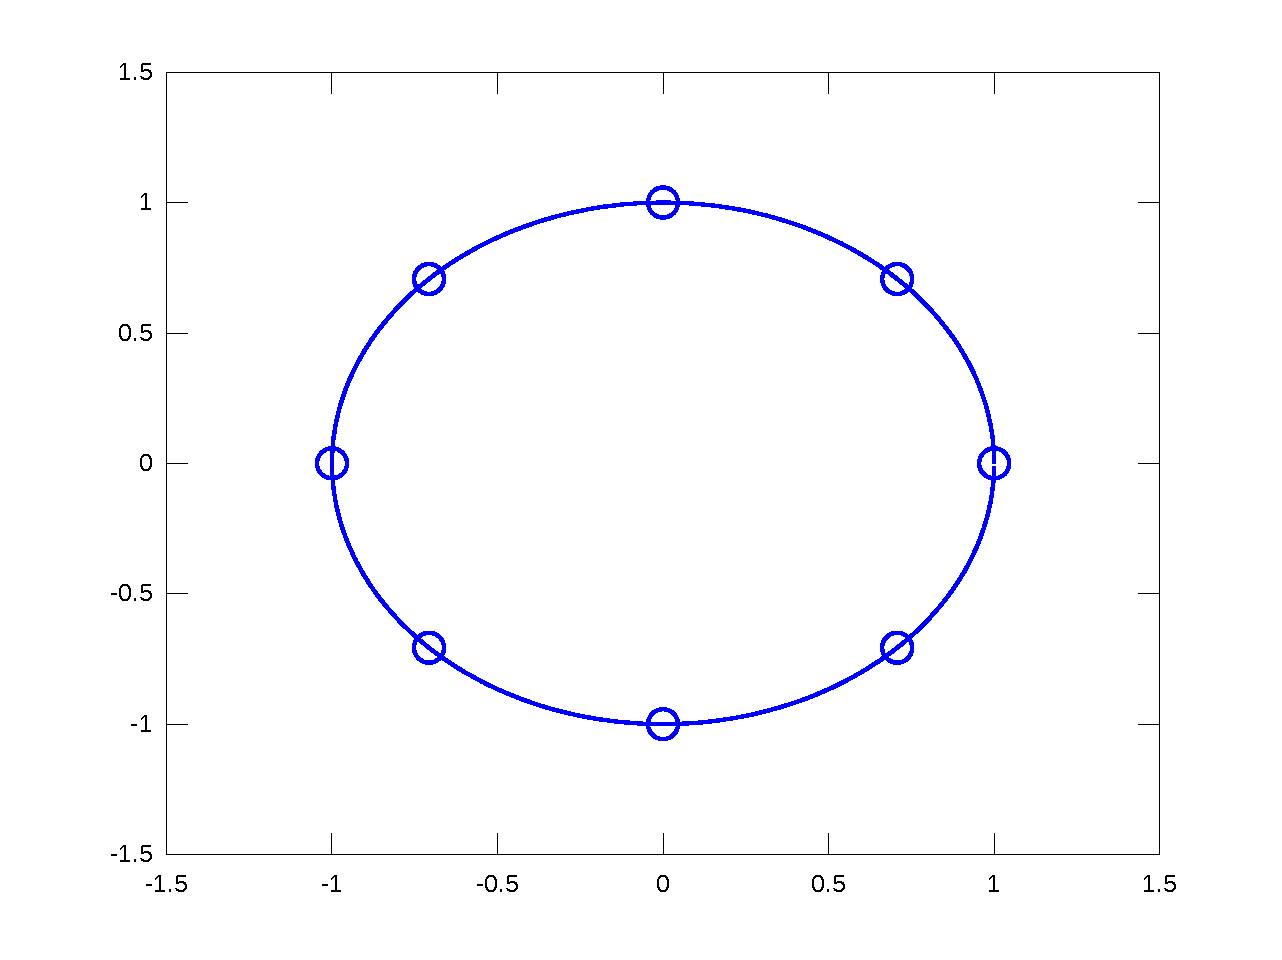
\includegraphics[width=0.48\textwidth]{\plotdir/ICF2_2}
	  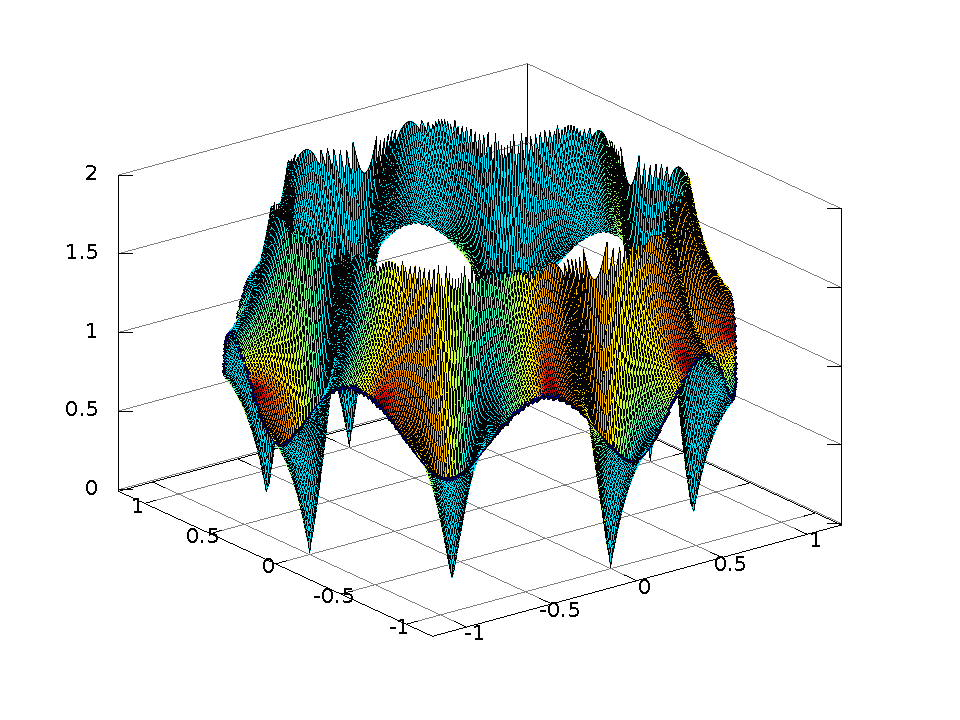
\includegraphics[width=0.48\textwidth]{\plotdir/ICF2_3}
		\caption{Disposizione degli zeri sul piano zeta per un filtro comb inverso di ordine 8\label{fig: icomb 8 zeroes}}
	\end{center}
\end{figure}

Come si pu\`o notare, gli zeri appaiono a $R^{L} e^{i 2 pi \times 0/L} = 1$,
$R^{L} e^{i 2 \pi \times 1/L} = R^{L} e^{i 2 \pi / 8} = R^{L} e^{i \pi / 4} = 0.707 + i 0.707$,
$R^{L} e^{i 2 \pi \times 2 /L} = R^{L} e^{i 4 \pi / 8} = e^{i \pi /2} = i$, ecc.
La Fig.\vref{fig: icomb 8 bode} invece mostra che la fase \`e per lo pi\`u
lineare, con gli shift di fase che accadono al passaggio dagli zeri della
magnitudine.

\begin{figure}[htbp]
	\begin{center}
	  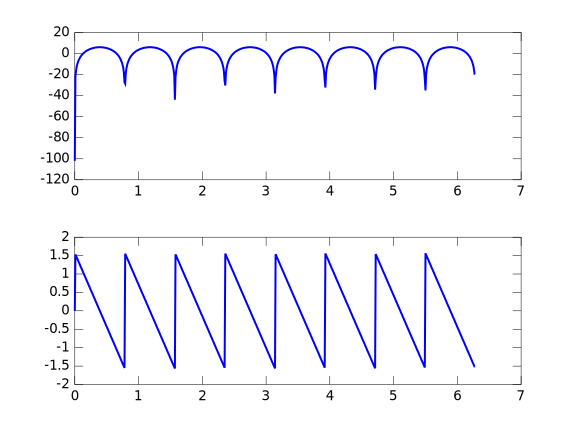
\includegraphics[width=0.8\textwidth]{\plotdir/ICF2_1}
	  \caption{Risposta in frequenza e in fase di un filtro comb inverso di ordine 8\label{fig: icomb 8 bode}}
	\end{center}
\end{figure}

\needspace{20\baselineskip}
Lo script \emph{octave} che produce questi plot \`e riportato qui di seguito:
\verbatiminput{\plotdir/ICF2.m}

Attenzione: un errore comune \`e quello di invertire l'ordine dei coefficienti nel
passare l'argomento alla funzione {\tt roots()} di \emph{matlab/octave}.
L'ordine \`e \ul{dal coefficiente pi\`u alto a quello pi\`u basso} (zero
incluso).

% esempio di signal cancellation
 % inverse comb filters

\chapter{La progettazione dei filtri FIR\label{chap:filter design}}

%
% $Id: filter_design.tex 14 2014-02-04 22:36:30Z nicb $
%
% cap.12
%
\svnInfo $Id: filter_design.tex 14 2014-02-04 22:36:30Z nicb $

\section{Introduzione alla progettazione di filtri FIR\label{sec: filter design introduction}}
%
% tecniche di design: ottimizzazione iterativa
%                   forme chiuse
%

Il problema sostanziale nel progettare i filtri \`e quello di trovare i giusti
coefficienti per raggiungere la migliore approssimazione alla ``risposta ideale''
che si desidera ottenere. In linea generale, la ``risposta ideale'' non \`e
ottenibile direttamente perch\'e si tratta di una funzione discontinua (che
non \`e realizzabile con un polinomio. Il problema \`e rappresentato in
fig.\vref{fig:ideal vs real}.
\begin{figure}[htbp]
	\begin{center}
		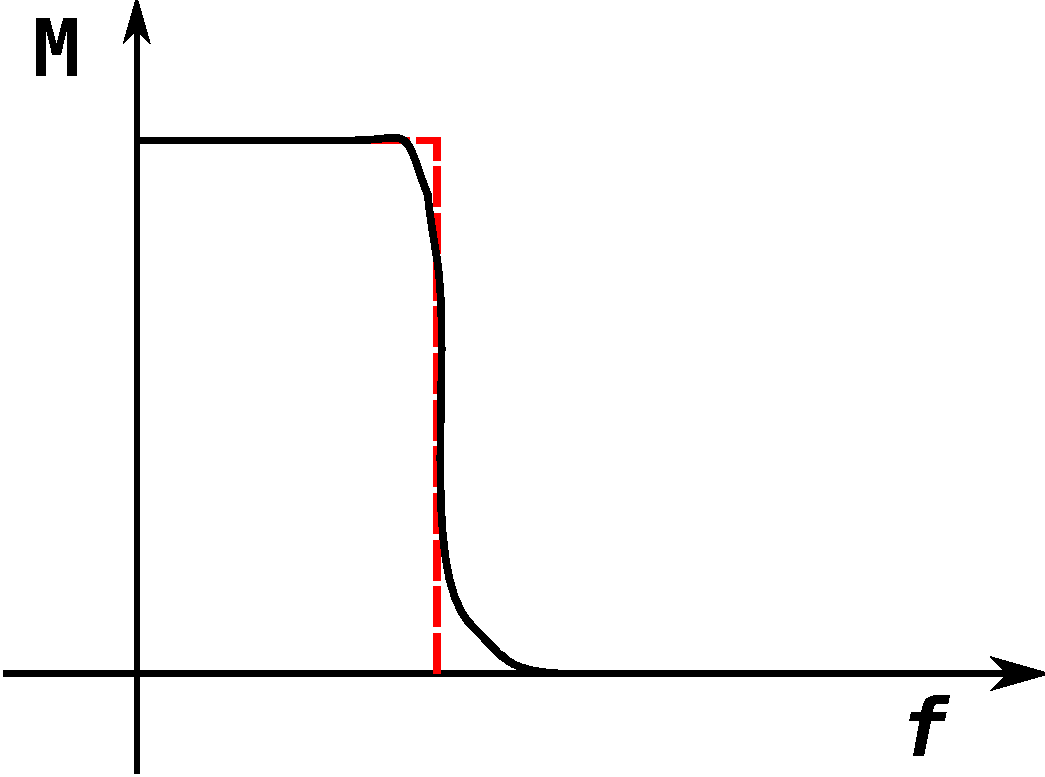
\includegraphics[width=0.75\textwidth]{\imagedir/ideal_vs_real}
		\caption{La risposta ideale di un filtro (in rosso) e la sua risposta reale\label{fig:ideal vs real}}
	\end{center}
\end{figure}

Ci sono varie soluzioni per ottenere questi coefficienti, e queste soluzioni
si applicano meglio a certi tipi di filtri che ad altri.
In alcuni casi \`e possibile (o necessario) trovare delle ``forme chiuse''
(vale a dire delle equazioni matematiche finite) per individuare i
coefficienti, mentre in altri casi \`e possibile trovarli attraverso una
``ottimizzazione iterativa'' (vale a dire ottenendo prima una approssimazione
mediocre per poi migliorarla a discrezione).

I coefficienti dei filtri FIR si trovano pi\`u facilmente attraverso
quest'ultima tecnica (ottimizzazione iterativa).

%
% ordine del filtro e simmetria dei coefficienti (0, N-1 per N coefficienti, N-1 ordine)
%

Ricordiamo che la forma dei filtri FIR \`e specificata da un'equazione del
tipo:

\begin{equation}
	y_t = a_0 x_t + a_1 x_{t-1} + a_2 x_{t-2} + \dots + a_{n-1} x_{t-(n-1)}
\end{equation}

Il primo coefficiente \`e il coefficiente $0$, quindi l'ultimo coefficiente di
un filtro di lunghezza $n$ \`e $n-1$. La sua funzione di trasferimento \`e

\begin{equation}
	H(z) = a_0 + a_1 z^{-1} + a_2 z^{-2} + \dots + a_{n-1} z^{-(n-1)}
\end{equation}

Considerando che la risposta $y_t$ deve essere una risposta reale, possiamo
semplificare la nostra progettazione utilizzando un numero pari di
coefficienti. Questi coefficienti distribuiranno gli zeri sul piano zeta in
posizioni complesse--coniugate ed il risultato sar\`a quindi reale.
Il problema \`e che abbiamo un coefficiente $0$, e che quindi se usiamo filtri
di lunghezza pari avremo una asimmetria intorno all'asse dei numeri reali.
Dobbiamo quindi utilizzare una lunghezza \emph{dispari} per ottenere un numero
\emph{pari} di coefficienti simmetrici (e un coefficiente direttamente
sull'asse reale -- che quindi sar\`a un numero reale).

Ad esempio, se usiamo un filtro di lunghezza 5, avremo la funzione di
trasferimento

\begin{equation}\label{eqn: fir order five}
		H(z) = a_0 + a_1 z^{-1} + a_2 z^{-2} + a_3 z^{-3} + a_4 z^{-4}
\end{equation}

Il trucco standard \`e quello di mettere a fattore una potenza di $z$
corrispondente al \emph{ritardo medio} del nostro filtro. Nel caso
dell'equazione \ref{eqn: fir order five} il ritardo medio sar\`a $z^{-2}$.
L'equazione viene cos\`i riscritta

\begin{equation}\label{eqn: fir order five rewritten}
	H(z) = z^{-2} \left [ a_0 z^{2} + a_1 z + a_2 + a_3 z^{-1} + a_4 z^{-2} \right ]
\end{equation}

La risposta in frequenza corrispondente viene ottenuta, come sempre,
sostituendo $z = e^{i \omega}$.

\begin{equation}\label{eqn: fir order five freq response}
	H(\omega) = e^{-i2\omega} \left [ a_0 e^{i2\omega} + a_1 e^{i\omega} + a_2 + a_3 e^{-i\omega} + a_4 e^{-i2\omega} \right ]
\end{equation}

Abbiamo visto che coefficienti simmetrici producono una risposta in fase
lineare. Daremo quindi per scontato che $a_0 = a_4$ e $a_1 = a_3$.
Ma 

\begin{equation}
	a_0 ( e^{i 2 \omega} + e^{-i 2 \omega} ) = 2 a_0 cos(2 \omega)
\end{equation}

e

\begin{equation}
	a_1 ( e^{i \omega} + e^{-i \omega} ) = 2 a_1 cos(\omega)
\end{equation}

Quindi:

\begin{equation}\label{eqn: fir order five freq response rewritten}
	H(\omega) = e^{-i2\omega} \left [ a_2 + 2 a_1 cos \omega + 2 a_0 cos (2 \omega) \right ]
\end{equation}

Come si pu\`o notare, la parte fra parentesi quadre \`e \emph{reale}, e il
fattore complesso che la moltiplica altro non \`e che un ritardo
``complessivo'' di due campioni. Questo fattore non influisce sulla
magnitudine del filtro, perch\'e il modulo di $e^{-i 2 \omega}$ \`e $1$.

Per semplificare ulteriormente, possiamo utilizzare dei coefficienti $c_i$ in
ordine ascendente, riscrivendo cos\`i l'equazione \ref{eqn: fir order five freq response rewritten} come:

\begin{equation}\label{eqn: fir order five freq response rewritten 2}
  \hat{H}(\omega) = e^{i2\omega} H(\omega) = c_0 + c_1 cos \omega + c_2 cos (2 \omega)
\end{equation}

dove $c_0 = a_2$, $c_1 = 2 a_1$ e $c_2 = 2 a_0$. Il ritardo lo abbiamo
spostato a sinistra dell'equazione (dove in realt\`a \`e un anticipo piuttosto
che un ritardo).

La nuova risposta in frequenza $\hat{H}(\omega)$ incorpora quindi il ritardo
generale ed \`e esclusivamente reale.
Per semplificarci la vita ulteriormente, diamo per scontato che la lunghezza
del filtro sia sempre un intero dispari.
\`E facile notare che la forma generale dell'eq.\ref{eqn: fir order five freq response rewritten}
\`e

\begin{equation}\label{eqn: fir rewritten general form}
  \hat{H}(\omega) = e^{im\omega} H(\omega) = c_0 + c_1 cos \omega + c_2 cos (2 \omega) + \dots + c_m cos (m \omega)
\end{equation}

dove $m = 1/2 (n - 1)$.
Dal momento che contiamo sempre a partire da $0$, ci saranno $m + 1 = 1/2 (n + 1)$ coefficienti $c$.
Dato che i coefficienti $a$ sono simmetrici, $m + 1$ saranno i coefficienti
con i quali avremo a che fare.

Ultima cosa: dato che a noi interessa soprattutto la magnitudine della
risposta in frequenza, considereremo quindi la parte destra dell'equazione
\ref{eqn: fir rewritten general form} senza il ritardo.
Questa parte sar\`a costituita da valori reali sia positivi che negativi.
Volendo, possiamo interpretare la magnitudine negativa come un shift di fase di $\pi$
radianti.

Riassumendo: quando disegniamo un filtro FIR, diamo per scontato che questi
filtri abbiano un numero dispari di termini ($n$)
i cui coefficienti siano simmetrici intorno al termine centrale.
La risposta in frequenza \`e quindi determinata dalla serie (solo di valori
reali) dei coseni dell'eq.\ref{eqn: fir rewritten general form} con $m = 1/2 ( n + 1 ) $
incognite $c_i$.
Il problema della progettazione del filtro si riduce cos\`i alla scelta di
questi coefficienti $c_i$ in modo da soddisfare le specifiche date.

%
% aggiungere qui la definizione di passband, stopband e boundaries
%

La chiave della soluzione \`e legata al fatto che la risposta in frequenza
della serie dei coseni in eq.\ref{eqn: fir rewritten general form} \`e una
funzione \emph{lineare} con coefficienti sconosciuti.
Facciamo un esempio volutamente molto semplice per illustrare l'idea.
Supponiamo di voler progettare un filtro di lunghezza $3$ -- nel quale dovremo
scegliere appunto due soli coefficienti.
Potremmo dare le specifiche seguenti:

\begin{compactenum}

	\item nella parte \emph{passband}, il confine superiore della funzione non
					deve superare il valore $1.05$, ossia:

					\begin{equation}
						\hat{H} (\omega) = c_0 + c_1 cos \omega \leq 1.05
					\end{equation}

	
	\item nella parte \emph{passband}, il confine inferiore della funzione non
					non deve essere meno di $0.95$, ossia:

					\begin{equation}
						\hat{H} (\omega) = c_0 + c_1 cos \omega \geq 0.95
					\end{equation}

	\item e cos\`i via.

\end{compactenum}

Si mettono insieme tante ``restrizioni'' di questo tipo suddividendo la
funzione in tanti punti e poi si cercano i coefficienti $c_i$ che
soddisfino simultaneamente tutti questi punti. Se, ad esempio, suddividiamo la
parte \emph{passband} in 500 punti e la parte \emph{stopband} in altri 500
punti, avremo 1000 ``restrizioni'' da rispettare simultaneamente.
La soluzione sembra molto difficile, ma in realt\`a la matematica degli anni '40 
ha trovato degli algoritmi (detti di \emph{programmazione lineare})
per risolvere questo tipo di problemi.
Questo tipo di problemi si chiama \emph{minimax} perch\'e vogliamo
\emph{massimizzare la distanza minima} per ogni ``restrizione''.

A questo punto, tenendo conto del fatto che i coefficienti che si stanno
cercando sono quelli di una serie di coseni, possiamo utilizzare una serie di
Fourier di soli coseni con le ampiezze che soddisfino le restrizioni poste. I
coefficienti della serie dovranno essere opportunamente ``finestrati'' per
evitare il fenomeno del \emph{ripple} nella parte \emph{passband} e nella
parte \emph{band--reject}.
La lunghezza del filtro sar\`a basata sulle restrizioni poste sulla larghezza
di banda della transizione.

%
% scelta dell'ordine del filtro
%


% %
% $Id: z_transform.tex 14 2014-02-04 22:36:30Z nicb $
%

\svnInfo $Id: z_transform.tex 14 2014-02-04 22:36:30Z nicb $

\section{La trasformata \emph{zeta}}

\begin{itemize}

  \item funzioni di variabile complessa: come sono fatte?
    funzioni di mappatura tra un piano e un altro;
    esempi: $\frac{1}{z}$, $\frac{1}{z^2}$, ecc.

  \item trasformata $z$:
	
		 \begin{equation}
	      X ( z ) = \sum_{n = 0}{x(n) z^{-n}}\
		 \end{equation}
		 
    quando $z = e^{i \omega t}$ la trasformata z d\`a la risposta in freq.

  \item perch\'e si usa? perch\'e trasforma la sequenza di campioni in
    un polinomio, e un polinomio si pu\`o trattare matematicamente
    (== \`e possibile vedere cosa ``fa'' su tutto il piano z)

  \item radice di un polinomio $\Rightarrow$ quando il polinomio va a zero


\end{itemize}


\bibliographystyle{apalike}
\bibliography{CSEDSMI}

\end{document}
